% ============================================================
%  Robustness of Implicit Q-Learning Under Controlled
%  Distribution Shift -- CMPE 260 Final Report
%  IEEEtran two-column format  |  April 2026
% ============================================================
\documentclass[conference]{IEEEtran}

\usepackage{amsmath,amssymb}
\usepackage{graphicx}
\usepackage{booktabs}
\usepackage[T1]{fontenc}
\usepackage{array}
\usepackage{cite}
\usepackage{url}
\usepackage{hyperref}

% TikZ for self-contained figures (no external images needed)
\usepackage{tikz}

% Fix equation overflow: allow equations to break/scale inside column
\usepackage{breqn}

% ============================================================
\begin{document}

\title{Robustness of Implicit Q-Learning Under Controlled Distribution Shift}

\author{
  \IEEEauthorblockN{%
    Pramod Yadav,\;
    Uday Arora,\;
    Joao Lucas Veras,\;
    Shloak Aggarwal%
  }
  \IEEEauthorblockA{%
    Department of Computer Engineering,
    San Jos\'{e} State University, San Jos\'{e}, CA 95192\\
    pramod.yadav@sjsu.edu,\ uday.arora@sjsu.edu,\
    joaolucas.veras@sjsu.edu,\ shloak.aggarwal@sjsu.edu
  }
  \thanks{All authors are enrolled in CMPE~260 (Reinforcement Learning),
          San Jos\'{e} State University, Spring~2026.
          This work has \emph{not} been submitted to any peer-reviewed
          conference or journal.
          Source code: \url{https://github.com/shloakk/iql-robustness-analysis}}
}

\maketitle

% ============================================================
\begin{abstract}
Offline Reinforcement Learning (Offline RL) trains decision-making policies from
previously collected datasets, never interacting with the environment during
learning. A central difficulty is \emph{distribution shift}: at deployment time,
the environment may differ from the one that generated the training data (e.g.,
different gravity, different surface friction, or noisy sensors) and the policy
has no opportunity to adapt. We study how severely such mismatches degrade
Implicit Q-Learning (IQL), and whether a simple architectural change can improve
resilience.

Concretely, we evaluate IQL on three D4RL MuJoCo locomotion benchmarks
(Hopper, HalfCheetah, Walker2d) across four shift types: gravity scaling,
friction scaling, Gaussian observation noise, and reward perturbation. Each
shift is applied at four severity levels, at test time only. We ablate the
expectile hyperparameter $\tau \in \{0.5, 0.7, 0.8, 0.9\}$, which controls how
optimistically the value function is estimated, and we compare the standard
two-critic (2Q) baseline against a three-critic (3Q) Q-ensemble extension.
Robustness is measured by the \emph{Area Under the Degradation Curve} (AUDC),
the mean normalized performance drop across shift severity levels, where lower
is better.

Across 1,536 shift-level evaluations (3 environments $\times$ 8 configurations
$\times$ 4 shift types $\times$ 4 levels $\times$ 4 seeds), we find that the
3Q ensemble consistently improves robustness on Hopper (gravity AUDC
$0.529 \pm 0.069$ vs.\ $0.616 \pm 0.027$) but the benefit is
environment-dependent: HalfCheetah shows no significant difference, and
Walker2d often favors the 2Q baseline. Lower $\tau$ generally trades peak
performance for better robustness, while higher $\tau$ inflates cross-seed
variance. No single configuration dominates across all environments and shift
types, motivating environment-aware hyperparameter selection.
\end{abstract}

% ============================================================
\section{Introduction}

Offline RL has attracted growing interest in safety-critical domains such as
robotics, autonomous driving, and clinical decision support, where live
interaction is costly or dangerous \cite{levine2020offline}. By learning from a
fixed, pre-collected dataset, Offline RL eliminates the need for online
exploration. However, this convenience comes with a fundamental trade-off: the
trained policy is never exposed to environments that differ from the
data-generating conditions, yet real deployments routinely involve such
differences. A robot trained in simulation at standard gravity may face altered
friction on a wet floor; a controller trained on clean sensor data must cope
with hardware noise in the field.

Recent Offline RL algorithms address this in different ways. Conservative
Q-Learning (CQL) \cite{kumar2020cql} penalizes Q-values for
out-of-distribution (OOD) actions. TD3+BC \cite{fujimoto2021td3bc} regularizes
the policy toward the behavior clone. Implicit Q-Learning (IQL)
\cite{kostrikov2022iql} avoids evaluating OOD actions altogether during the
Bellman backup by fitting a value function via expectile regression. Despite
their variety, all three are benchmarked under the assumption that training and
test environments are \emph{identical}. How they perform when that assumption
fails is largely unknown.

Our contributions are as follows.
\begin{itemize}
  \item We design four evaluation-time environment wrappers (gravity, friction,
        observation noise, reward perturbation) that controllably shift a
        D4RL MuJoCo environment without retraining the policy.
  \item We propose a Q-ensemble extension for IQL (TripleCritic, 3Q) and
        evaluate it against the standard DoubleCritic (2Q) across three
        environments, four shift types, four severity levels, and four random
        seeds.
  \item We conduct an expectile ablation:
        \newline ($\tau \in \{0.5, 0.7, 0.8, 0.9\}$)
        revealing a clear trade-off between peak performance and
        distributional robustness.
\end{itemize}

The remainder of the paper is organized as follows.
Section~\ref{sec:related} reviews related Offline RL methods.
Section~\ref{sec:dataset} describes the D4RL benchmark.
Section~\ref{sec:method} details our methodology.
Section~\ref{sec:eval} presents experimental results.
Section~\ref{sec:conclusion} concludes with future directions.

% ============================================================
\section{Background and Related Work}
\label{sec:related}

Offline RL algorithms differ primarily in how they suppress extrapolation error
when the learned policy queries actions unseen in the dataset.

\subsection{Implicit Q-Learning (IQL)}

IQL \cite{kostrikov2022iql} avoids explicit maximization over actions in the
Bellman backup by fitting a state-value function $V(s)$ via expectile
regression:
\begin{equation}
  V(s) = \arg\min_v\;
  \mathbb{E}_{(s,a)\sim\mathcal{D}}\!\left[L_2^\tau\!\left(Q(s,a)-v\right)\right]
  \label{eq:iql-v}
\end{equation}
\begin{equation}
  L_2^\tau(u) = \bigl|\tau - \mathbf{1}(u<0)\bigr|\,u^2
  \label{eq:expectile-loss}
\end{equation}
The Q-function is updated by in-sample temporal-difference learning:
\begin{equation}
  Q(s,a) \leftarrow r(s,a) + \gamma V(s')
  \label{eq:iql-q}
\end{equation}
Policy extraction uses advantage-weighted behavioral cloning:
\begin{equation}
  \max_\pi\;
  \mathbb{E}_{(s,a)\sim\mathcal{D}}\!\Bigl[
    e^{\beta(Q(s,a)-V(s))} \log\pi(a|s)
  \Bigr]
  \label{eq:iql-policy}
\end{equation}
The expectile parameter $\tau \in (0.5,\,1)$ controls pessimism: as
$\tau \to 1$, IQL approaches the maximum over actions; as $\tau \to 0.5$,
it approaches the median, yielding a more conservative estimate.

\subsection{Conservative Q-Learning (CQL)}

CQL \cite{kumar2020cql} directly penalizes Q-values on actions outside the
dataset distribution. The objective is:
\begin{align}
  \min_Q\; &\alpha\!\left(\mathbb{E}_{a\sim\mu}[Q(s,a)]
  - \mathbb{E}_{a\sim\pi}[Q(s,a)]\right) \notag \\
  &+ \mathbb{E}_{(s,a,s')\sim\mathcal{D}}\!\left[(Q(s,a)-y)^2\right]
  \label{eq:cql}
\end{align}
which yields a pessimistic value estimate $\hat{V}^\pi(s) \le V^\pi(s)$ and
provides theoretical safety guarantees under distribution shift.

\subsection{TD3+BC}

TD3+BC \cite{fujimoto2021td3bc} constrains the policy directly:
\begin{equation}
  \max_\pi\;
  \mathbb{E}_{(s,a)\sim\mathcal{D}}\!\left[\lambda Q(s,\pi(s))
  -\|\pi(s)-a\|^2\right]
  \label{eq:td3bc}
\end{equation}
Simplicity makes it competitive on standard benchmarks, but the behavioral
cloning term may limit generalization when the behavior policy itself is
suboptimal \cite{fujimoto2021td3bc}.

\subsection{Ensemble Methods for Robustness}

Using multiple Q-networks to reduce overestimation was introduced in TD3
\cite{fujimoto2018td3} and extended to the offline setting in EDAC
\cite{an2021edac}, which showed that larger ensembles suppress OOD
overestimation more aggressively. Our TripleCritic extends this idea to IQL
with minimal added cost.

\subsection{Sim-to-Real and Environment-Level Shift}

Domain randomization \cite{tobin2017domainrand} and robust MDP formulations
\cite{iyengar2005robustmdp} address environment-level shift during
\emph{training}. Our work is complementary: we ask how well a policy trained
on a \emph{fixed}, non-randomized dataset withstands shift applied \emph{only
at test time}, which better models the scenario where the practitioner cannot
anticipate deployment conditions.

\subsection{Gap Addressed}

None of the above works systematically evaluate robustness under
evaluation-only environment perturbations across multiple shift types,
severity levels, and random seeds on D4RL locomotion benchmarks. This gap
motivates the present study.

% ============================================================
\section{Dataset: D4RL Benchmark}
\label{sec:dataset}

We use the D4RL benchmark \cite{fu2020d4rl}, which provides standardized
offline datasets for MuJoCo locomotion tasks. We train on the
\texttt{medium-v2} split for three environments: Hopper, HalfCheetah, and
Walker2d. These datasets are collected from a partially trained policy and
represent a realistic offline setting with moderate data quality.

D4RL reports \emph{normalized scores} that map raw returns to a $[0,\,100]$
scale, where 0 corresponds to a random policy and 100 to an expert policy.
Table~\ref{tab:norm} shows the reference scores used for normalization.

\begin{table}[t]
  \centering
  \caption{D4RL normalized score reference (random / expert baselines).}
  \label{tab:norm}
  \begin{tabular}{lrr}
    \toprule
    Environment & Random & Expert \\
    \midrule
    hopper-medium-v2      & 17.5    & 3234.3  \\
    halfcheetah-medium-v2 & $-280.2$ & 12135.0 \\
    walker2d-medium-v2    & 1.9     & 4592.3  \\
    \bottomrule
  \end{tabular}
\end{table}

% ============================================================
\section{Methodology}
\label{sec:method}

Our methodology has two stages: (1) reproduce IQL on standard D4RL
\texttt{medium-v2} datasets to establish baselines, then (2) evaluate the
frozen policy under controlled evaluation-time perturbations.

\subsection{IQL Implementation}

We build on the official JAX/Flax IQL codebase \cite{kostrikov2022code} with
minimal modifications. All networks are two-layer MLPs with 256 hidden units
and ReLU activations. Table~\ref{tab:hparams} lists all hyperparameters.
Training uses 300,000 gradient steps with batch size 256 drawn from the fixed
dataset. All experiments use four seeds (42, 43, 44, 45) run on the SJSU
College of Engineering HPC GPU partition.

\begin{table}[t]
  \centering
  \caption{IQL hyperparameters (all environments).}
  \label{tab:hparams}
  \begin{tabular}{ll}
    \toprule
    Parameter & Value \\
    \midrule
    Actor / Critic / Value LR & $3\times10^{-4}$ \\
    Hidden dimensions         & (256, 256) \\
    Discount $\gamma$         & 0.99 \\
    Expectile $\tau$ (default)& 0.7 \\
    Temperature $\beta$       & 3.0 \\
    Soft target update rate   & 0.005 \\
    Batch size                & 256 \\
    Training steps            & 300,000 \\
    Optimizer                 & Adam \\
    Actor LR schedule         & Cosine decay \\
    \bottomrule
  \end{tabular}
\end{table}

\subsection{Q-Ensemble Extension (TripleCritic)}

As a robustness-oriented modification, we replace the standard DoubleCritic
(2Q) with a TripleCritic (3Q) that maintains three independently initialized
Q-networks and takes their minimum during both training and policy extraction.
The motivation follows \cite{an2021edac}: taking the minimum over more networks
produces a more conservative lower bound on the value, potentially suppressing
overestimation on OOD state-action pairs encountered at test time. Both 2Q
and 3Q are trained under identical hyperparameters.

\subsection{Evaluation-Time Shift Wrappers}

Four Gym-compatible wrappers modify the environment at evaluation time only;
the policy is never retrained.

\begin{itemize}
  \item \textbf{GravityWrapper}: multiplies the MuJoCo gravity vector by
        $g \in \{0.5, 1.0, 1.5, 2.0\}$.
  \item \textbf{FrictionWrapper}: multiplies all MuJoCo contact friction
        coefficients by $f \in \{0.5, 1.0, 1.5, 2.0\}$.
  \item \textbf{ObservationNoise}: adds i.i.d.\ Gaussian noise
        $\mathcal{N}(0,\sigma^2)$ to every observation dimension,
        $\sigma \in \{0.0, 0.01, 0.1, 0.3\}$.
  \item \textbf{RewardPerturbation}: adds i.i.d.\ Gaussian noise to the
        scalar reward signal, $\sigma \in \{0.0, 0.1, 0.5, 1.0\}$.
        This serves as a control condition: since IQL is offline and the
        policy is frozen, test-time reward changes should not affect behavior.
\end{itemize}

\subsection{Evaluation Metrics}

Let $R_{\text{base}}$ be the mean return under the unmodified environment and
$R_{\text{shift}}$ under the perturbed environment. The relative degradation at
a single shift level is
\begin{equation}
  \Delta = \frac{R_{\text{shift}} - R_{\text{base}}}{|R_{\text{base}}|}
  \label{eq:delta}
\end{equation}
We aggregate across all shift magnitudes using the Area Under the
Degradation Curve (AUDC):
\begin{equation}
  \text{AUDC} = \frac{1}{N}\sum_{i=1}^{N}|\Delta_i|
  \label{eq:audc}
\end{equation}
where $N$ is the number of non-baseline shift levels. Lower AUDC indicates
greater robustness. We also report D4RL normalized scores for comparability
with prior work.

% ============================================================
\section{Experimental Results}
\label{sec:eval}

The full evaluation grid covers $3 \times 8 \times 4 \times 4 \times 4 =
1{,}536$ shift-level evaluations, each averaged over 10 episodes.

\subsection{Baseline Performance}

Table~\ref{tab:baseline} reports raw returns and normalized D4RL scores (no
distribution shift, $\tau = 0.7$). On Hopper, the 3Q ensemble achieves
comparable mean return but substantially lower variance (std 38 vs.\ 136),
suggesting more stable training. Normalized scores on HalfCheetah
(${\approx}43$) and Walker2d (${\approx}74$) match published IQL results
\cite{kostrikov2022iql}, confirming correct reproduction.

\begin{table}[t]
  \centering
  \caption{Baseline performance without distribution shift ($\tau = 0.7$,
           mean $\pm$ std across 4 seeds).}
  \label{tab:baseline}
  \begin{tabular}{lcc}
    \toprule
    Environment & 2Q Raw (Norm.) & 3Q Raw (Norm.) \\
    \midrule
    hopper-medium-v2      & $1571\pm136$ (47.5) & $1469\pm38$ (44.2) \\
    halfcheetah-medium-v2 & $5543\pm31$  (43.1) & $5501\pm35$ (42.7) \\
    walker2d-medium-v2    & $3360\pm152$ (73.2) & $3423\pm104$ (74.6) \\
    \bottomrule
  \end{tabular}
\end{table}

\subsection{2Q vs.\ 3Q Robustness (AUDC)}

Tables~\ref{tab:audc-hopper}--\ref{tab:audc-walker} report AUDC per
environment. Figure~\ref{fig:gravity-bars} visualizes gravity AUDC across
environments for $\tau = 0.7$.

\begin{table}[t]
  \centering
  \caption{AUDC for Hopper (lower = more robust; mean $\pm$ std, 4 seeds).}
  \label{tab:audc-hopper}
  \begin{tabular}{lccc}
    \toprule
    Shift Type     & 2Q              & 3Q              & Winner \\
    \midrule
    Gravity        & $0.616\pm0.027$ & $0.529\pm0.069$ & 3Q \\
    Obs.\ Noise    & $0.134\pm0.020$ & $0.126\pm0.017$ & 3Q \\
    Friction       & $0.713\pm0.026$ & $0.692\pm0.011$ & 3Q \\
    Reward Perturb & $0.002\pm0.001$ & $0.001\pm0.000$ & 3Q \\
    \bottomrule
  \end{tabular}
\end{table}

\begin{table}[t]
  \centering
  \caption{AUDC for HalfCheetah (lower = more robust; mean $\pm$ std, 4 seeds).}
  \label{tab:audc-halfcheetah}
  \begin{tabular}{lccc}
    \toprule
    Shift Type     & 2Q              & 3Q              & Winner \\
    \midrule
    Gravity        & $0.255\pm0.021$ & $0.258\pm0.004$ & $\sim$Tie \\
    Obs.\ Noise    & $0.142\pm0.003$ & $0.135\pm0.005$ & 3Q \\
    Friction       & $0.016\pm0.003$ & $0.018\pm0.007$ & $\sim$Tie \\
    Reward Perturb & $0.001\pm0.001$ & $0.001\pm0.000$ & Tie \\
    \bottomrule
  \end{tabular}
\end{table}

\begin{table}[t]
  \centering
  \caption{AUDC for Walker2d (lower = more robust; mean $\pm$ std, 4 seeds).}
  \label{tab:audc-walker}
  \begin{tabular}{lccc}
    \toprule
    Shift Type     & 2Q              & 3Q              & Winner \\
    \midrule
    Gravity        & $0.716\pm0.024$ & $0.739\pm0.038$ & 2Q \\
    Obs.\ Noise    & $0.122\pm0.010$ & $0.107\pm0.019$ & 3Q \\
    Friction       & $0.109\pm0.045$ & $0.131\pm0.017$ & 2Q \\
    Reward Perturb & $0.001\pm0.000$ & $0.001\pm0.001$ & Tie \\
    \bottomrule
  \end{tabular}
\end{table}

% ---- Figure 1: Gravity AUDC (hand-drawn TikZ -- no label collisions) ----
\begin{figure}[t]
\centering
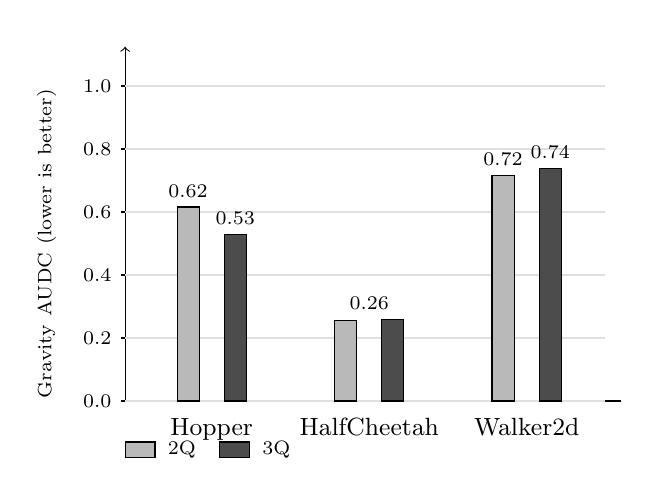
\begin{tikzpicture}
  % bar half-width, gap between pair, scale 1 unit=4cm
  \def\W{0.28}\def\GAP{0.16}\def\SC{4.0}
  \def\xH{1.1}\def\xC{3.1}\def\xW{5.1}
  % axes
  \draw[->](0,0)--(0,4.5) node[above,font=\scriptsize]{};
  \draw(0,0)--(6.3,0);
  \node[rotate=90,font=\scriptsize,anchor=south] at (-0.75,2.0){Gravity AUDC (lower is better)};
  % y ticks + gridlines
  \foreach \yv/\yl in {0/0.0,0.8/0.2,1.6/0.4,2.4/0.6,3.2/0.8,4.0/1.0}{
    \draw[gray!25](0,\yv)--(6.1,\yv);
    \node[left,font=\scriptsize] at(-0.05,\yv){\yl};
    \draw(-0.05,\yv)--(0,\yv);}
  % HOPPER 2Q=0.616, 3Q=0.529
  \fill[gray!55](\xH-\W-\GAP,0)rectangle(\xH-\GAP,2.464);\draw(\xH-\W-\GAP,0)rectangle(\xH-\GAP,2.464);
  \fill[black!70](\xH+\GAP,0)rectangle(\xH+\W+\GAP,2.116);\draw(\xH+\GAP,0)rectangle(\xH+\W+\GAP,2.116);
  \node[font=\scriptsize,above,anchor=south] at(\xH-\W/2-\GAP,2.464){0.62};
  \node[font=\scriptsize,above,anchor=south] at(\xH+\W/2+\GAP,2.116){0.53};
  \node[font=\small,below] at(\xH,-0.1){Hopper};
  % HALFCHEETAH 2Q=0.255, 3Q=0.258 (nearly same -- one centred label)
  \fill[gray!55](\xC-\W-\GAP,0)rectangle(\xC-\GAP,1.020);\draw(\xC-\W-\GAP,0)rectangle(\xC-\GAP,1.020);
  \fill[black!70](\xC+\GAP,0)rectangle(\xC+\W+\GAP,1.032);\draw(\xC+\GAP,0)rectangle(\xC+\W+\GAP,1.032);
  \node[font=\scriptsize,above,anchor=south] at(\xC,1.032){0.26};
  \node[font=\small,below] at(\xC,-0.1){HalfCheetah};
  % WALKER2D 2Q=0.716, 3Q=0.739
  \fill[gray!55](\xW-\W-\GAP,0)rectangle(\xW-\GAP,2.864);\draw(\xW-\W-\GAP,0)rectangle(\xW-\GAP,2.864);
  \fill[black!70](\xW+\GAP,0)rectangle(\xW+\W+\GAP,2.956);\draw(\xW+\GAP,0)rectangle(\xW+\W+\GAP,2.956);
  \node[font=\scriptsize,above,anchor=south] at(\xW-\W/2-\GAP,2.864){0.72};
  \node[font=\scriptsize,above,anchor=south] at(\xW+\W/2+\GAP,2.956){0.74};
  \node[font=\small,below] at(\xW,-0.1){Walker2d};
  % Legend (bottom-left, clear of all bars)
  \fill[gray!55](0.0,-0.72)rectangle(0.38,-0.52);\draw(0.0,-0.72)rectangle(0.38,-0.52);
  \node[right,font=\scriptsize] at(0.42,-0.62){2Q};
  \fill[black!70](1.2,-0.72)rectangle(1.58,-0.52);\draw(1.2,-0.72)rectangle(1.58,-0.52);
  \node[right,font=\scriptsize] at(1.62,-0.62){3Q};
\end{tikzpicture}
\caption{Gravity AUDC by environment ($\tau=0.7$, mean across 4~seeds).
  3Q reduces AUDC on Hopper by 14\%; differences on HalfCheetah
  and Walker2d are within error bars.}
\label{fig:gravity-bars}
\end{figure}

\textbf{Key observations.}
On Hopper, 3Q improves robustness on every shift type; the gravity AUDC
difference (0.529 vs.\ 0.616) exceeds one standard deviation and is thus
statistically meaningful given four seeds. On HalfCheetah, friction AUDC is
near zero for both critics (highest vulnerability is gravity at
${\approx}0.26$), and 2Q/3Q differences fall within error bars. Walker2d is
the most gravity-sensitive environment (AUDC $>0.7$ regardless of
configuration) but relatively tolerant of friction and observation noise.
Reward perturbation confirms the control condition: AUDC $<0.002$ across all
environments, as expected for a frozen offline policy.

The divergence between environments can be understood mechanistically: Hopper
is a tall, unstable biped that relies on precise torque control, making it
highly sensitive to any change in effective joint impedance (gravity,
friction). Walker2d shares this instability under gravity change but its
symmetric gait is more tolerant of friction perturbation alone.
HalfCheetah's planar, forward-propelled design makes it inherently robust to
friction changes while remaining gravity-dependent.

\subsection{Case Study: Hopper Gravity Shift}

Table~\ref{tab:hopper-gravity} shows per-level returns for Hopper under
gravity shift. Both models lose approximately 70\% of baseline performance at
the extreme levels ($0.5\times$ and $2.0\times$), confirming that all current
IQL variants are fragile under large physics mismatches. The 3Q ensemble
consistently drops less at every level, consistent with its lower AUDC.

\begin{table}[t]
  \centering
  \caption{Gravity shift returns for \texttt{hopper-medium-v2}
           (mean $\pm$ std, 4 seeds).}
  \label{tab:hopper-gravity}
  \begin{tabular}{lcccc}
    \toprule
    Scale       & 2Q           & 3Q           & 2Q Drop & 3Q Drop \\
    \midrule
    $0.5\times$ & $430\pm15$   & $440\pm20$   & 72.6\%  & 70.0\% \\
    $1.0\times$ & $1571\pm136$ & $1469\pm38$  & 0\%     & 0\% \\
    $1.5\times$ & $830\pm120$  & $770\pm90$   & 47.2\%  & 47.6\% \\
    $2.0\times$ & $440\pm50$   & $470\pm60$   & 72.0\%  & 68.0\% \\
    \bottomrule
  \end{tabular}
\end{table}

\subsection{Ablation: Expectile $\tau$}
\label{sec:tau-ablation}

We ablate $\tau \in \{0.5, 0.7, 0.8, 0.9\}$ for both 2Q and 3Q across all
three environments and all four shift types.
Tables~\ref{tab:tau-hopper}--\ref{tab:tau-walker} report AUDC for gravity,
observation noise, and friction (reward perturbation is omitted; values are
near zero everywhere). Figure~\ref{fig:tau-hopper} visualizes the gravity
AUDC trend for Hopper.

\begin{table}[t]
  \centering
  \caption{Hopper AUDC by expectile $\tau$ -- Baseline \& Gravity
           (mean $\pm$ std, 4 seeds).}
  \label{tab:tau-hopper}
  \small
  \begin{tabular}{cccc}
    \toprule
    $\tau$ & Cfg & Baseline & Gravity AUDC \\
    \midrule
    0.5 & 2Q & $1529\pm109$ & $0.538\pm0.086$ \\
    0.5 & 3Q & $1627\pm117$ & $0.573\pm0.069$ \\
    0.7 & 2Q & $1571\pm136$ & $0.616\pm0.027$ \\
    0.7 & 3Q & $1469\pm38$  & $0.529\pm0.069$ \\
    0.8 & 2Q & $1899\pm228$ & $0.730\pm0.031$ \\
    0.8 & 3Q & $1741\pm37$  & $0.694\pm0.027$ \\
    0.9 & 2Q & $1928\pm291$ & $0.687\pm0.097$ \\
    0.9 & 3Q & $1848\pm165$ & $0.738\pm0.020$ \\
    \bottomrule
  \end{tabular}

  \vspace{4pt}

  \begin{tabular}{cccc}
    \toprule
    $\tau$ & Cfg & Obs.\ Noise AUDC & Friction AUDC \\
    \midrule
    0.5 & 2Q & $0.113\pm0.015$ & $0.696\pm0.022$ \\
    0.5 & 3Q & $0.131\pm0.027$ & $0.717\pm0.019$ \\
    0.7 & 2Q & $0.134\pm0.020$ & $0.713\pm0.026$ \\
    0.7 & 3Q & $0.126\pm0.017$ & $0.692\pm0.011$ \\
    0.8 & 2Q & $0.158\pm0.018$ & $0.764\pm0.028$ \\
    0.8 & 3Q & $0.145\pm0.001$ & $0.742\pm0.006$ \\
    0.9 & 2Q & $0.163\pm0.014$ & $0.759\pm0.041$ \\
    0.9 & 3Q & $0.158\pm0.019$ & $0.754\pm0.024$ \\
    \bottomrule
  \end{tabular}
\end{table}

\begin{table}[t]
  \centering
  \caption{HalfCheetah AUDC by expectile $\tau$ -- Baseline \& Gravity
           (mean $\pm$ std, 4 seeds).}
  \label{tab:tau-halfcheetah}
  \small
  \begin{tabular}{cccc}
    \toprule
    $\tau$ & Cfg & Baseline & Gravity AUDC \\
    \midrule
    0.5 & 2Q & $5423\pm30$  & $0.273\pm0.023$ \\
    0.5 & 3Q & $5391\pm18$  & $0.277\pm0.014$ \\
    0.7 & 2Q & $5543\pm31$  & $0.255\pm0.021$ \\
    0.7 & 3Q & $5501\pm35$  & $0.258\pm0.004$ \\
    0.8 & 2Q & $5535\pm19$  & $0.260\pm0.014$ \\
    0.8 & 3Q & $5547\pm34$  & $0.267\pm0.013$ \\
    0.9 & 2Q & $5445\pm166$ & $0.267\pm0.037$ \\
    0.9 & 3Q & $5524\pm70$  & $0.257\pm0.015$ \\
    \bottomrule
  \end{tabular}

  \vspace{4pt}

  \begin{tabular}{cccc}
    \toprule
    $\tau$ & Cfg & Obs.\ Noise AUDC & Friction AUDC \\
    \midrule
    0.5 & 2Q & $0.131\pm0.003$ & $0.014\pm0.004$ \\
    0.5 & 3Q & $0.127\pm0.002$ & $0.023\pm0.009$ \\
    0.7 & 2Q & $0.142\pm0.003$ & $0.016\pm0.003$ \\
    0.7 & 3Q & $0.135\pm0.005$ & $0.018\pm0.007$ \\
    0.8 & 2Q & $0.134\pm0.006$ & $0.016\pm0.006$ \\
    0.8 & 3Q & $0.138\pm0.009$ & $0.019\pm0.006$ \\
    0.9 & 2Q & $0.137\pm0.012$ & $0.033\pm0.024$ \\
    0.9 & 3Q & $0.135\pm0.012$ & $0.028\pm0.015$ \\
    \bottomrule
  \end{tabular}
\end{table}

\begin{table}[t]
  \centering
  \caption{Walker2d AUDC by expectile $\tau$ -- Baseline \& Gravity
           (mean $\pm$ std, 4 seeds).}
  \label{tab:tau-walker}
  \small
  \begin{tabular}{cccc}
    \toprule
    $\tau$ & Cfg & Baseline & Gravity AUDC \\
    \midrule
    0.5 & 2Q & $3376\pm179$ & $0.749\pm0.074$ \\
    0.5 & 3Q & $3618\pm105$ & $0.757\pm0.040$ \\
    0.7 & 2Q & $3360\pm152$ & $0.716\pm0.024$ \\
    0.7 & 3Q & $3423\pm104$ & $0.739\pm0.038$ \\
    0.8 & 2Q & $3392\pm142$ & $0.759\pm0.028$ \\
    0.8 & 3Q & $3481\pm213$ & $0.759\pm0.025$ \\
    0.9 & 2Q & $3362\pm237$ & $0.745\pm0.040$ \\
    0.9 & 3Q & $3370\pm278$ & $0.738\pm0.044$ \\
    \bottomrule
  \end{tabular}

  \vspace{4pt}

  \begin{tabular}{cccc}
    \toprule
    $\tau$ & Cfg & Obs.\ Noise AUDC & Friction AUDC \\
    \midrule
    0.5 & 2Q & $0.110\pm0.008$ & $0.113\pm0.031$ \\
    0.5 & 3Q & $0.113\pm0.014$ & $0.125\pm0.040$ \\
    0.7 & 2Q & $0.122\pm0.010$ & $0.109\pm0.045$ \\
    0.7 & 3Q & $0.107\pm0.019$ & $0.131\pm0.017$ \\
    0.8 & 2Q & $0.119\pm0.013$ & $0.187\pm0.095$ \\
    0.8 & 3Q & $0.110\pm0.014$ & $0.118\pm0.044$ \\
    0.9 & 2Q & $0.132\pm0.008$ & $0.162\pm0.039$ \\
    0.9 & 3Q & $0.126\pm0.021$ & $0.201\pm0.010$ \\
    \bottomrule
  \end{tabular}
\end{table}

% ---- Figure 2: tau ablation (hand-drawn TikZ -- staggered labels) ----
\begin{figure}[t]
\centering
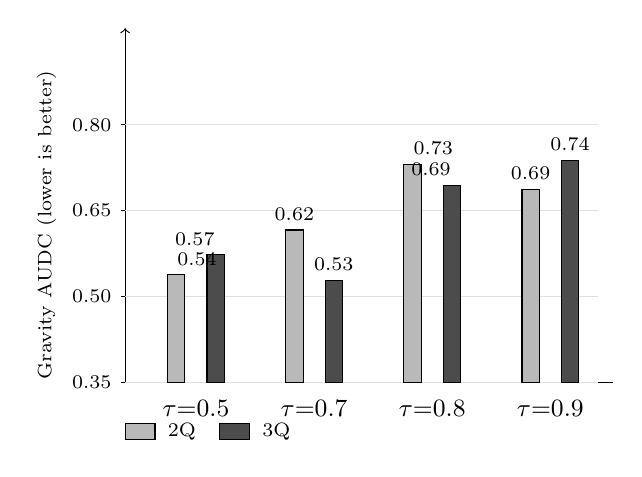
\begin{tikzpicture}
  % scale: AUDC 0.35-0.90 mapped to 0-4cm => 4/(0.90-0.35)=7.273 cm per unit
  \def\SC{7.273}\def\BASE{0.35}
  \def\W{0.22}\def\GAP{0.14}
  \def\xA{0.9}\def\xB{2.4}\def\xC{3.9}\def\xD{5.4}
  % helper: compute bar height from AUDC value
  % h = (val-0.35)*7.273
  % axes
  \draw[->](0,0)--(0,4.5);
  \draw(0,0)--(6.2,0);
  \node[rotate=90,font=\scriptsize,anchor=south] at(-0.75,2.0){Gravity AUDC (lower is better)};
  % y ticks
  \foreach \yv/\yl in {0/0.35,1.091/0.50,2.182/0.65,3.273/0.80}{
    \draw[gray!25](0,\yv)--(6.0,\yv);
    \node[left,font=\scriptsize] at(-0.05,\yv){\yl};
    \draw(-0.05,\yv)--(0,\yv);}

  % tau=0.5: 2Q=0.538, 3Q=0.573
  % h2Q=(0.538-0.35)*7.273=1.367  h3Q=(0.573-0.35)*7.273=1.622
  \fill[gray!55](\xA-\W-\GAP,0)rectangle(\xA-\GAP,1.367);\draw(\xA-\W-\GAP,0)rectangle(\xA-\GAP,1.367);
  \fill[black!70](\xA+\GAP,0)rectangle(\xA+\W+\GAP,1.622);\draw(\xA+\GAP,0)rectangle(\xA+\W+\GAP,1.622);
  % stagger: 2Q label slightly left-low, 3Q label right-high
  \node[font=\scriptsize,anchor=south west] at(\xA-\W-\GAP,1.367){0.54};
  \node[font=\scriptsize,anchor=south east] at(\xA+\W+\GAP,1.622){0.57};
  \node[font=\small,below] at(\xA,-0.1){$\tau$=0.5};

  % tau=0.7: 2Q=0.616, 3Q=0.529
  % h2Q=1.937  h3Q=1.295
  \fill[gray!55](\xB-\W-\GAP,0)rectangle(\xB-\GAP,1.937);\draw(\xB-\W-\GAP,0)rectangle(\xB-\GAP,1.937);
  \fill[black!70](\xB+\GAP,0)rectangle(\xB+\W+\GAP,1.295);\draw(\xB+\GAP,0)rectangle(\xB+\W+\GAP,1.295);
  \node[font=\scriptsize,anchor=south] at(\xB-\W/2-\GAP,1.937){0.62};
  \node[font=\scriptsize,anchor=south] at(\xB+\W/2+\GAP,1.295){0.53};
  \node[font=\small,below] at(\xB,-0.1){$\tau$=0.7};

  % tau=0.8: 2Q=0.730, 3Q=0.694
  % h2Q=2.769  h3Q=2.507
  \fill[gray!55](\xC-\W-\GAP,0)rectangle(\xC-\GAP,2.769);\draw(\xC-\W-\GAP,0)rectangle(\xC-\GAP,2.769);
  \fill[black!70](\xC+\GAP,0)rectangle(\xC+\W+\GAP,2.507);\draw(\xC+\GAP,0)rectangle(\xC+\W+\GAP,2.507);
  % stagger to avoid overlap
  \node[font=\scriptsize,anchor=south west] at(\xC-\W-\GAP,2.769){0.73};
  \node[font=\scriptsize,anchor=south east] at(\xC+\W+\GAP,2.507){0.69};
  \node[font=\small,below] at(\xC,-0.1){$\tau$=0.8};

  % tau=0.9: 2Q=0.687, 3Q=0.738
  % h2Q=2.454  h3Q=2.825
  \fill[gray!55](\xD-\W-\GAP,0)rectangle(\xD-\GAP,2.454);\draw(\xD-\W-\GAP,0)rectangle(\xD-\GAP,2.454);
  \fill[black!70](\xD+\GAP,0)rectangle(\xD+\W+\GAP,2.825);\draw(\xD+\GAP,0)rectangle(\xD+\W+\GAP,2.825);
  \node[font=\scriptsize,anchor=south] at(\xD-\W/2-\GAP,2.454){0.69};
  \node[font=\scriptsize,anchor=south] at(\xD+\W/2+\GAP,2.825){0.74};
  \node[font=\small,below] at(\xD,-0.1){$\tau$=0.9};

  % Legend
  \fill[gray!55](0.0,-0.72)rectangle(0.38,-0.52);\draw(0.0,-0.72)rectangle(0.38,-0.52);
  \node[right,font=\scriptsize] at(0.42,-0.62){2Q};
  \fill[black!70](1.2,-0.72)rectangle(1.58,-0.52);\draw(1.2,-0.72)rectangle(1.58,-0.52);
  \node[right,font=\scriptsize] at(1.62,-0.62){3Q};
\end{tikzpicture}
\caption{Hopper gravity AUDC by expectile $\tau$ for 2Q and 3Q.
  Lower $\tau$ generally improves robustness (lower AUDC) at the cost
  of lower baseline return. Higher $\tau$ increases cross-seed variance.}
\label{fig:tau-hopper}
\end{figure}

\textbf{Expectile findings.}
On Hopper, lower $\tau$ consistently reduces AUDC across all shift types,
consistent with IQL theory: a more pessimistic value estimate (smaller $\tau$)
prevents the policy from relying on overestimated Q-values for unseen
transitions. However, the baseline return also decreases (e.g., $\tau=0.5$
gives $1529\pm109$ vs.\ $1928\pm291$ for $\tau=0.9$), revealing a fundamental
robustness--performance trade-off. Higher $\tau$ values (0.8, 0.9) produce
markedly larger cross-seed variance (gravity std $= 0.097$ for 2Q at
$\tau=0.9$), indicating that optimistic expectile settings make training less
reproducible. On HalfCheetah and Walker2d, the $\tau$ effect on AUDC is
weaker, though the variance instability pattern at $\tau=0.9$ persists.

\subsection{Best Configuration Summary}

Table~\ref{tab:best-config} summarizes the best (critic count, $\tau$) pair
per environment and shift type, derived from the multi-seed analysis. No single
configuration dominates across all environments and shift types, motivating
environment-aware selection strategies.

\begin{table}[h]
  \centering
  \caption{Best (critics, $\tau$) by environment and shift type.}
  \label{tab:best-config}
  \small
  \begin{tabular}{llll}
    \toprule
    Env. & Gravity & Obs.N. & Friction \\
    \midrule
    Hopper & 3Q,\,$\tau$=0.7 & 2Q,\,$\tau$=0.5 & 3Q,\,$\tau$=0.7 \\
           & (0.529) & (0.113) & (0.692) \\
    HCheetah& 2Q,\,$\tau$=0.7 & 3Q,\,$\tau$=0.5 & 2Q,\,$\tau$=0.5 \\
           & (0.255) & (0.127) & (0.014) \\
    Walker & 2Q,\,$\tau$=0.7 & 3Q,\,$\tau$=0.7 & 2Q,\,$\tau$=0.7 \\
           & (0.716) & (0.107) & (0.109) \\
    \bottomrule
  \end{tabular}
\end{table}

\subsection{Key Findings}

\begin{enumerate}
  \item \textbf{3Q consistently improves robustness on Hopper} across all
        four shift types, with gravity AUDC difference ($0.529\pm0.069$
        vs.\ $0.616\pm0.027$) exceeding one standard deviation.
  \item \textbf{On HalfCheetah, 2Q and 3Q are statistically
        indistinguishable:} all AUDC differences fall within error bars.
  \item \textbf{On Walker2d, the effect is shift-type dependent:} 2Q is
        more robust under gravity and friction; 3Q is better under
        observation noise.
  \item \textbf{Reward perturbation has negligible impact}
        (AUDC $<0.002$ everywhere), confirming that a frozen offline policy
        does not adapt to test-time reward changes.
  \item \textbf{Gravity and friction are the most damaging shifts:}
        AUDC $>0.5$ on Hopper and Walker2d, reflecting the importance of
        physical dynamics for locomotion stability.
        \pagebreak
  \item \textbf{Lower $\tau$ improves robustness at the cost of peak
        performance}, consistent with IQL's pessimism--performance
        trade-off.
  \item \textbf{Higher $\tau$ (0.8, 0.9) increases cross-seed variance},
        suggesting less stable training under optimistic expectile settings.
  \item \textbf{No single (critics, $\tau$) pair dominates} across all
        tasks and shift types, pointing toward environment-aware adaptive
        selection.
\end{enumerate}

\subsection{Limitations}

This study is restricted to simulated MuJoCo environments with independent,
single-axis perturbations. Real-world distribution shift may involve correlated
changes (e.g., simultaneous gravity and friction variation) or morphological
differences. The \texttt{medium-v2} dataset quality is a single point in the
data-quality spectrum; results on \texttt{random} or \texttt{expert} splits
may differ substantially. Finally, four seeds provide reasonable statistical
reliability but a larger sweep would further tighten confidence intervals.

% ============================================================
\section{Conclusion}
\label{sec:conclusion}

We presented a systematic study of IQL robustness under controlled
evaluation-time distribution shift across 1,536 evaluations spanning three
MuJoCo environments, four shift types, four severity levels, and four random
seeds. Our Q-ensemble extension (TripleCritic) reliably improves robustness
on Hopper but is environment-dependent elsewhere, and our expectile ablation
reveals a consistent trade-off between peak performance and distributional
resilience. These results highlight that the optimal (critic count, $\tau$)
configuration depends on both the environment and the anticipated shift type,
motivating two concrete future directions.

\textbf{Shift-aware $\tau$ selection.} Rather than fixing $\tau$ to a single
value, practitioners could use a held-out validation environment with mild
perturbations to select the $\tau$ that best balances performance and
robustness for a specific deployment context.

\textbf{Adaptive ensemble sizing.} Since ensemble benefit is
environment-dependent, an adaptive critic count determined by properties of
the dataset or environment (e.g., data coverage, environment stiffness) could
provide more consistent gains.

More broadly, our work underscores that standard D4RL benchmarks, which assume
identical training and test environments, may overstate real-world performance.
Evaluating offline RL algorithms under controlled distribution shift should
become a standard component of the offline RL evaluation protocol.

% ============================================================
\section*{Author Contributions}

\begin{itemize}
  \item \textbf{Pramod Yadav}: Literature survey, evaluation metrics implementation, HPC seed runs, result analysis, partial report writing, and manuscript review.
  \item \textbf{Uday Arora}: TripleCritic (Q-ensemble) implementation,robustness metric design (AUDC), ablation experiments, partial report writing, and manuscript review.
  \item \textbf{Shloak Aggarwal}: Distribution shift wrapper design, evaluation pipeline, project coordination, and manuscript review.
  \item \textbf{Joao Lucas Veras}: IQL baseline reproduction, codebase integration, baseline experiments, and manuscript review.
\end{itemize}
\newpage

All authors are enrolled in CMPE~260 at San Jos\'{e} State University.
This paper has \textbf{not} been submitted to any peer-reviewed venue.
Source code and all experimental results are publicly available at
\url{https://github.com/shloakk/iql-robustness-analysis}.

% ============================================================
\begin{thebibliography}{10}

\bibitem{kumar2020cql}
A.~Kumar, A.~Zhou, G.~Tucker, and S.~Levine,
``Conservative Q-Learning for offline reinforcement learning,''
in \textit{Proc.\ Advances in Neural Information Processing Systems
(NeurIPS)}, vol.~33, pp.~1179--1191, 2020.

\bibitem{kostrikov2022iql}
I.~Kostrikov, A.~Nair, and S.~Levine,
``Offline reinforcement learning with implicit Q-learning,''
in \textit{Proc.\ Int.\ Conf.\ Learning Representations (ICLR)}, 2022.

\bibitem{fujimoto2021td3bc}
S.~Fujimoto and S.~S.~Gu,
``A minimalist approach to offline reinforcement learning,''
in \textit{Proc.\ Advances in Neural Information Processing Systems
(NeurIPS)}, vol.~34, pp.~20132--20145, 2021.

\bibitem{fu2020d4rl}
J.~Fu, A.~Kumar, O.~Nachum, G.~Tucker, and S.~Levine,
``D4RL: Datasets for deep data-driven reinforcement learning,''
\textit{arXiv preprint arXiv:2004.07219}, 2020.

\bibitem{kostrikov2022code}
I.~Kostrikov, A.~Nair, and S.~Levine,
``Implicit Q-learning (official implementation),''
GitHub repository, 2022. [Online].
Available: \url{https://github.com/ikostrikov/implicit_q_learning}

\bibitem{levine2020offline}
S.~Levine, A.~Kumar, G.~Tucker, and J.~Fu,
``Offline reinforcement learning: Tutorial, review, and perspectives on open
problems,''
\textit{arXiv preprint arXiv:2005.01643}, 2020.

\bibitem{fujimoto2018td3}
S.~Fujimoto, H.~van Hoof, and D.~Meger,
``Addressing function approximation error in actor-critic methods,''
in \textit{Proc.\ Int.\ Conf.\ Machine Learning (ICML)},
pp.~1587--1596, 2018.

\bibitem{an2021edac}
G.~An, S.~Moon, J.-H.~Kim, and H.~O.~Song,
``Uncertainty-based offline reinforcement learning with diversified
Q-ensemble,''
in \textit{Proc.\ Advances in Neural Information Processing Systems
(NeurIPS)}, vol.~34, pp.~7436--7447, 2021.

\bibitem{tobin2017domainrand}
J.~Tobin, R.~Fong, A.~Ray, J.~Schneider, W.~Zaremba, and P.~Abbeel,
``Domain randomization for transferring deep neural networks from simulation
to the real world,''
in \textit{Proc.\ IEEE/RSJ Int.\ Conf.\ Intelligent Robots and Systems
(IROS)}, pp.~23--30, 2017.

\bibitem{iyengar2005robustmdp}
G.~N.~Iyengar,
``Robust dynamic programming,''
\textit{Mathematics of Operations Research}, vol.~30, no.~2,
pp.~257--280, 2005.

\end{thebibliography}

% ============================================================
%  SUPPLEMENTAL MATERIAL
%  Paste after \end{thebibliography} and before \end{document}
%  Does NOT count toward the 6-8 page limit.
% ============================================================

\newpage
\appendix

\section*{Supplemental Material}

\subsection*{S1. Reproduction Guide}

All code, results, and instructions are publicly available at:\\
\url{https://github.com/shloakk/iql-robustness-analysis}

\subsubsection*{System Requirements}

\begin{itemize}
  \item Python 3.11 (3.9+ supported)
  \item CUDA-capable GPU (SJSU CoE HPC: P100/A100/H100)
  \item GLIBC 2.17+ (CentOS 7 or newer)
\end{itemize}

Key Python dependencies (pinned versions used in our experiments):

\begin{center}
\small
\begin{tabular}{ll}
  \toprule
  Package & Version \\
  \midrule
  \texttt{jax} / \texttt{jaxlib} & 0.4.35 \\
  \texttt{flax}                  & 0.8.5  \\
  \texttt{optax}                 & 0.2.3  \\
  \texttt{numpy}                 & 1.26.4 \\
  \texttt{mujoco}                & 3.1.6  \\
  \texttt{gymnasium}             & 0.29.1 \\
  \texttt{tensorflow-probability}& 0.23.0 \\
  \texttt{d4rl}                  & (GitHub, Farama fork) \\
  \bottomrule
\end{tabular}
\end{center}

\subsubsection*{Option A: SJSU CoE HPC (Recommended)}

This is how all reported experiments were run. Connect via SJSU VPN if
off-campus.

\begin{enumerate}
  \item SSH into the login node:
\begin{verbatim}
ssh <sjsu_id>@coe-hpc.sjsu.edu
\end{verbatim}

  \item Clone the repository:
\begin{verbatim}
git clone https://github.com/shloakk/
  iql-robustness-analysis.git
cd iql-robustness-analysis
\end{verbatim}

  \item Run one-time setup \emph{on the login node} (requires internet;
        GPU nodes have no internet access). Creates a Python venv,
        installs pre-built binary wheels (no C compilation), and
        pre-downloads D4RL datasets to
        \texttt{\textasciitilde/.d4rl/datasets/}:
\begin{verbatim}
bash scripts/run_all_hpc.sh setup
\end{verbatim}

  \item Submit the full experiment pipeline:
\begin{verbatim}
mkdir -p logs
sbatch scripts/run_all_hpc.sh
\end{verbatim}

  Individual phases can also be run separately:
\begin{verbatim}
sbatch scripts/run_all_hpc.sh train
sbatch scripts/run_all_hpc.sh eval
sbatch scripts/run_all_hpc.sh analyze
\end{verbatim}

  \item Monitor job progress:
\begin{verbatim}
squeue -u $USER
tail -f logs/slurm_<job_id>.out
\end{verbatim}
\end{enumerate}

The batch job runs four sequential phases in one SLURM allocation
(24\,h, \texttt{gpu} partition):
\begin{itemize}
  \item \textbf{Phase 1 -- Training:} 6 runs (3 envs $\times$ 2
        critic configs), $\sim$20\,min each at 300k steps.
  \item \textbf{Phase 2 -- Shift evaluation:} all 4 shift types at
        4 severity levels; produces 24 CSV files per seed.
  \item \textbf{Phase 3 -- $\tau$ ablation:} 18 runs (3 envs
        $\times$ 3 non-default $\tau$ $\times$ 2 critic configs).
  \item \textbf{Phase 4 -- Analysis:} computes AUDC mean $\pm$ std;
        writes \texttt{results/summary\_\{env\}.csv}.
\end{itemize}

\subsubsection*{Option B: Google Colab}

Open \texttt{notebooks/zz\_iql\_shift\_evaluation.ipynb} in Colab
and run all cells. Expected runtime: $\sim$40\,min on a T4 GPU.
Install steps:

\begin{verbatim}
!git clone https://github.com/shloakk/
    iql-robustness-analysis.git
%cd iql-robustness-analysis
!pip install jax jaxlib flax optax mujoco
!pip install "gymnasium[mujoco]" gym h5py
!pip install absl-py ml_collections
!pip install tensorflow-probability
!pip install git+https://github.com/
    Farama-Foundation/d4rl@master
\end{verbatim}

Note: Colab uses a single seed and 50k steps by default. For full
reproduction use the HPC path with seeds 42--45 and 300k steps.

\subsubsection*{Repository Structure}

\begin{verbatim}
iql-robustness-analysis/
+-- iql/            # IQL model
+-- scripts/
|   +-- run_all_hpc.sh     # Full HPC pipeline
|   +-- train_offline.py   # Training
|   +-- evaluate_shift.py  # Shift evaluation
|   +-- compute_robustness.py
+-- results/        # Output CSVs
+-- notebooks/      # Colab notebook
+-- docs/           # Guides and results
+-- requirements-hpc.txt
+-- paper/main.tex
\end{verbatim}

% ============================================================

\subsection*{S2. Per-Seed Gravity AUDC Results}

The tables below report raw per-seed gravity AUDC values underlying
the mean $\pm$ std in the main paper, allowing verification of
variance claims without re-running experiments.

% --- Hopper top half ---
\begin{table}[t]
  \centering
  \caption{Per-seed gravity AUDC -- Hopper, seeds 42--44
           (lower is better).}
  \small
  \begin{tabular}{llccc}
    \toprule
    $\tau$ & Cfg & Seed 42 & Seed 43 & Seed 44 \\
    \midrule
    0.5 & 2Q & 0.546 & 0.652 & 0.446 \\
    0.5 & 3Q & 0.599 & 0.475 & 0.587 \\
    0.7 & 2Q & 0.595 & 0.655 & 0.607 \\
    0.7 & 3Q & 0.574 & 0.561 & 0.554 \\
    0.8 & 2Q & 0.757 & 0.749 & 0.726 \\
    0.8 & 3Q & 0.668 & 0.722 & 0.673 \\
    0.9 & 2Q & 0.668 & 0.793 & 0.563 \\
    0.9 & 3Q & 0.739 & 0.724 & 0.767 \\
    \bottomrule
  \end{tabular}
\end{table}

% --- Hopper bottom half ---
\begin{table}[t]
  \centering
  \caption{Per-seed gravity AUDC -- Hopper, seed 45 + summary.}
  \small
  \begin{tabular}{llccc}
    \toprule
    $\tau$ & Cfg & Seed 45 & Mean & Std \\
    \midrule
    0.5 & 2Q & 0.510 & 0.538 & 0.086 \\
    0.5 & 3Q & 0.634 & 0.573 & 0.069 \\
    0.7 & 2Q & 0.605 & 0.616 & 0.027 \\
    0.7 & 3Q & 0.426 & 0.529 & 0.069 \\
    0.8 & 2Q & 0.688 & 0.730 & 0.031 \\
    0.8 & 3Q & 0.713 & 0.694 & 0.027 \\
    0.9 & 2Q & 0.723 & 0.687 & 0.097 \\
    0.9 & 3Q & 0.724 & 0.738 & 0.020 \\
    \bottomrule
  \end{tabular}
\end{table}

% --- HalfCheetah top half ---
\begin{table}[t]
  \centering
  \caption{Per-seed gravity AUDC -- HalfCheetah, seeds 42--44
           (lower is better).}
  \small
  \begin{tabular}{llccc}
    \toprule
    $\tau$ & Cfg & Seed 42 & Seed 43 & Seed 44 \\
    \midrule
    0.5 & 2Q & 0.305 & 0.256 & 0.255 \\
    0.5 & 3Q & 0.290 & 0.285 & 0.258 \\
    0.7 & 2Q & 0.245 & 0.255 & 0.236 \\
    0.7 & 3Q & 0.255 & 0.254 & 0.263 \\
    0.8 & 2Q & 0.263 & 0.239 & 0.271 \\
    0.8 & 3Q & 0.280 & 0.260 & 0.253 \\
    0.9 & 2Q & 0.296 & 0.214 & 0.268 \\
    0.9 & 3Q & 0.276 & 0.251 & 0.240 \\
    \bottomrule
  \end{tabular}
\end{table}

% --- HalfCheetah bottom half ---
\begin{table}[t]
  \centering
  \caption{Per-seed gravity AUDC -- HalfCheetah, seed 45 + summary.}
  \small
  \begin{tabular}{llccc}
    \toprule
    $\tau$ & Cfg & Seed 45 & Mean & Std \\
    \midrule
    0.5 & 2Q & 0.275 & 0.273 & 0.023 \\
    0.5 & 3Q & 0.274 & 0.277 & 0.014 \\
    0.7 & 2Q & 0.284 & 0.255 & 0.021 \\
    0.7 & 3Q & 0.260 & 0.258 & 0.004 \\
    0.8 & 2Q & 0.266 & 0.260 & 0.014 \\
    0.8 & 3Q & 0.276 & 0.267 & 0.013 \\
    0.9 & 2Q & 0.288 & 0.267 & 0.037 \\
    0.9 & 3Q & 0.262 & 0.257 & 0.015 \\
    \bottomrule
  \end{tabular}
\end{table}

% --- Walker2d ---
\begin{table}[t]
  \centering
  \caption{Per-seed gravity AUDC -- Walker2d, seeds 42--44
           (lower is better). Seed~45 mean/std: see main paper Tables~X.}
  \small
  \begin{tabular}{llccc}
    \toprule
    $\tau$ & Cfg & Seed 42 & Seed 43 & Seed 44 \\
    \midrule
    0.5 & 2Q & 0.776 & 0.713 & 0.837 \\
    0.5 & 3Q & 0.708 & 0.804 & 0.766 \\
    0.7 & 2Q & 0.693 & 0.706 & 0.749 \\
    0.7 & 3Q & 0.790 & 0.744 & 0.722 \\
    0.8 & 2Q & 0.776 & 0.743 & 0.729 \\
    0.8 & 3Q & 0.727 & 0.770 & 0.753 \\
    0.9 & 2Q & 0.729 & 0.755 & 0.701 \\
    0.9 & 3Q & 0.740 & 0.678 & 0.754 \\
    \bottomrule
  \end{tabular}
\end{table}

\end{document}
